\section{Inteligência Artificial}

Inteligência artificial é uma técnica científica que simula o pensamento humano de forma que possa ser executado em uma máquina, podendo ser utilizada para criar soluções com uma linha de progressão parecida ao raciocínio lógico. Isto permite ao computador reconhecer e interpretar o mundo ao redor com imagens e textos, criando-se uma ampla área de atuação que otimiza tarefas antes só realizadas por seres humanos \space\cite{ia_aliada_ou_inimiga}.

% Esta área da ciência da computação é complexa por se tratar de uma representação cognitiva, se torna necessário usar uma base com diversas áreas científicas como psicologia, biologia, lógica matemática, linguística, engenharia, filosofia, entre outras. E pode ser usado para diversos problemas específicos como, por exemplo, definir as boas rotas para algum processo logístico \space\cite{ia_conceitos_aplicacoes}.

% \begin{figure}[ht]
% 	\caption{Diagrama de aprendizado de máquina}
% 	\centering % para centralizarmos a figura
% 	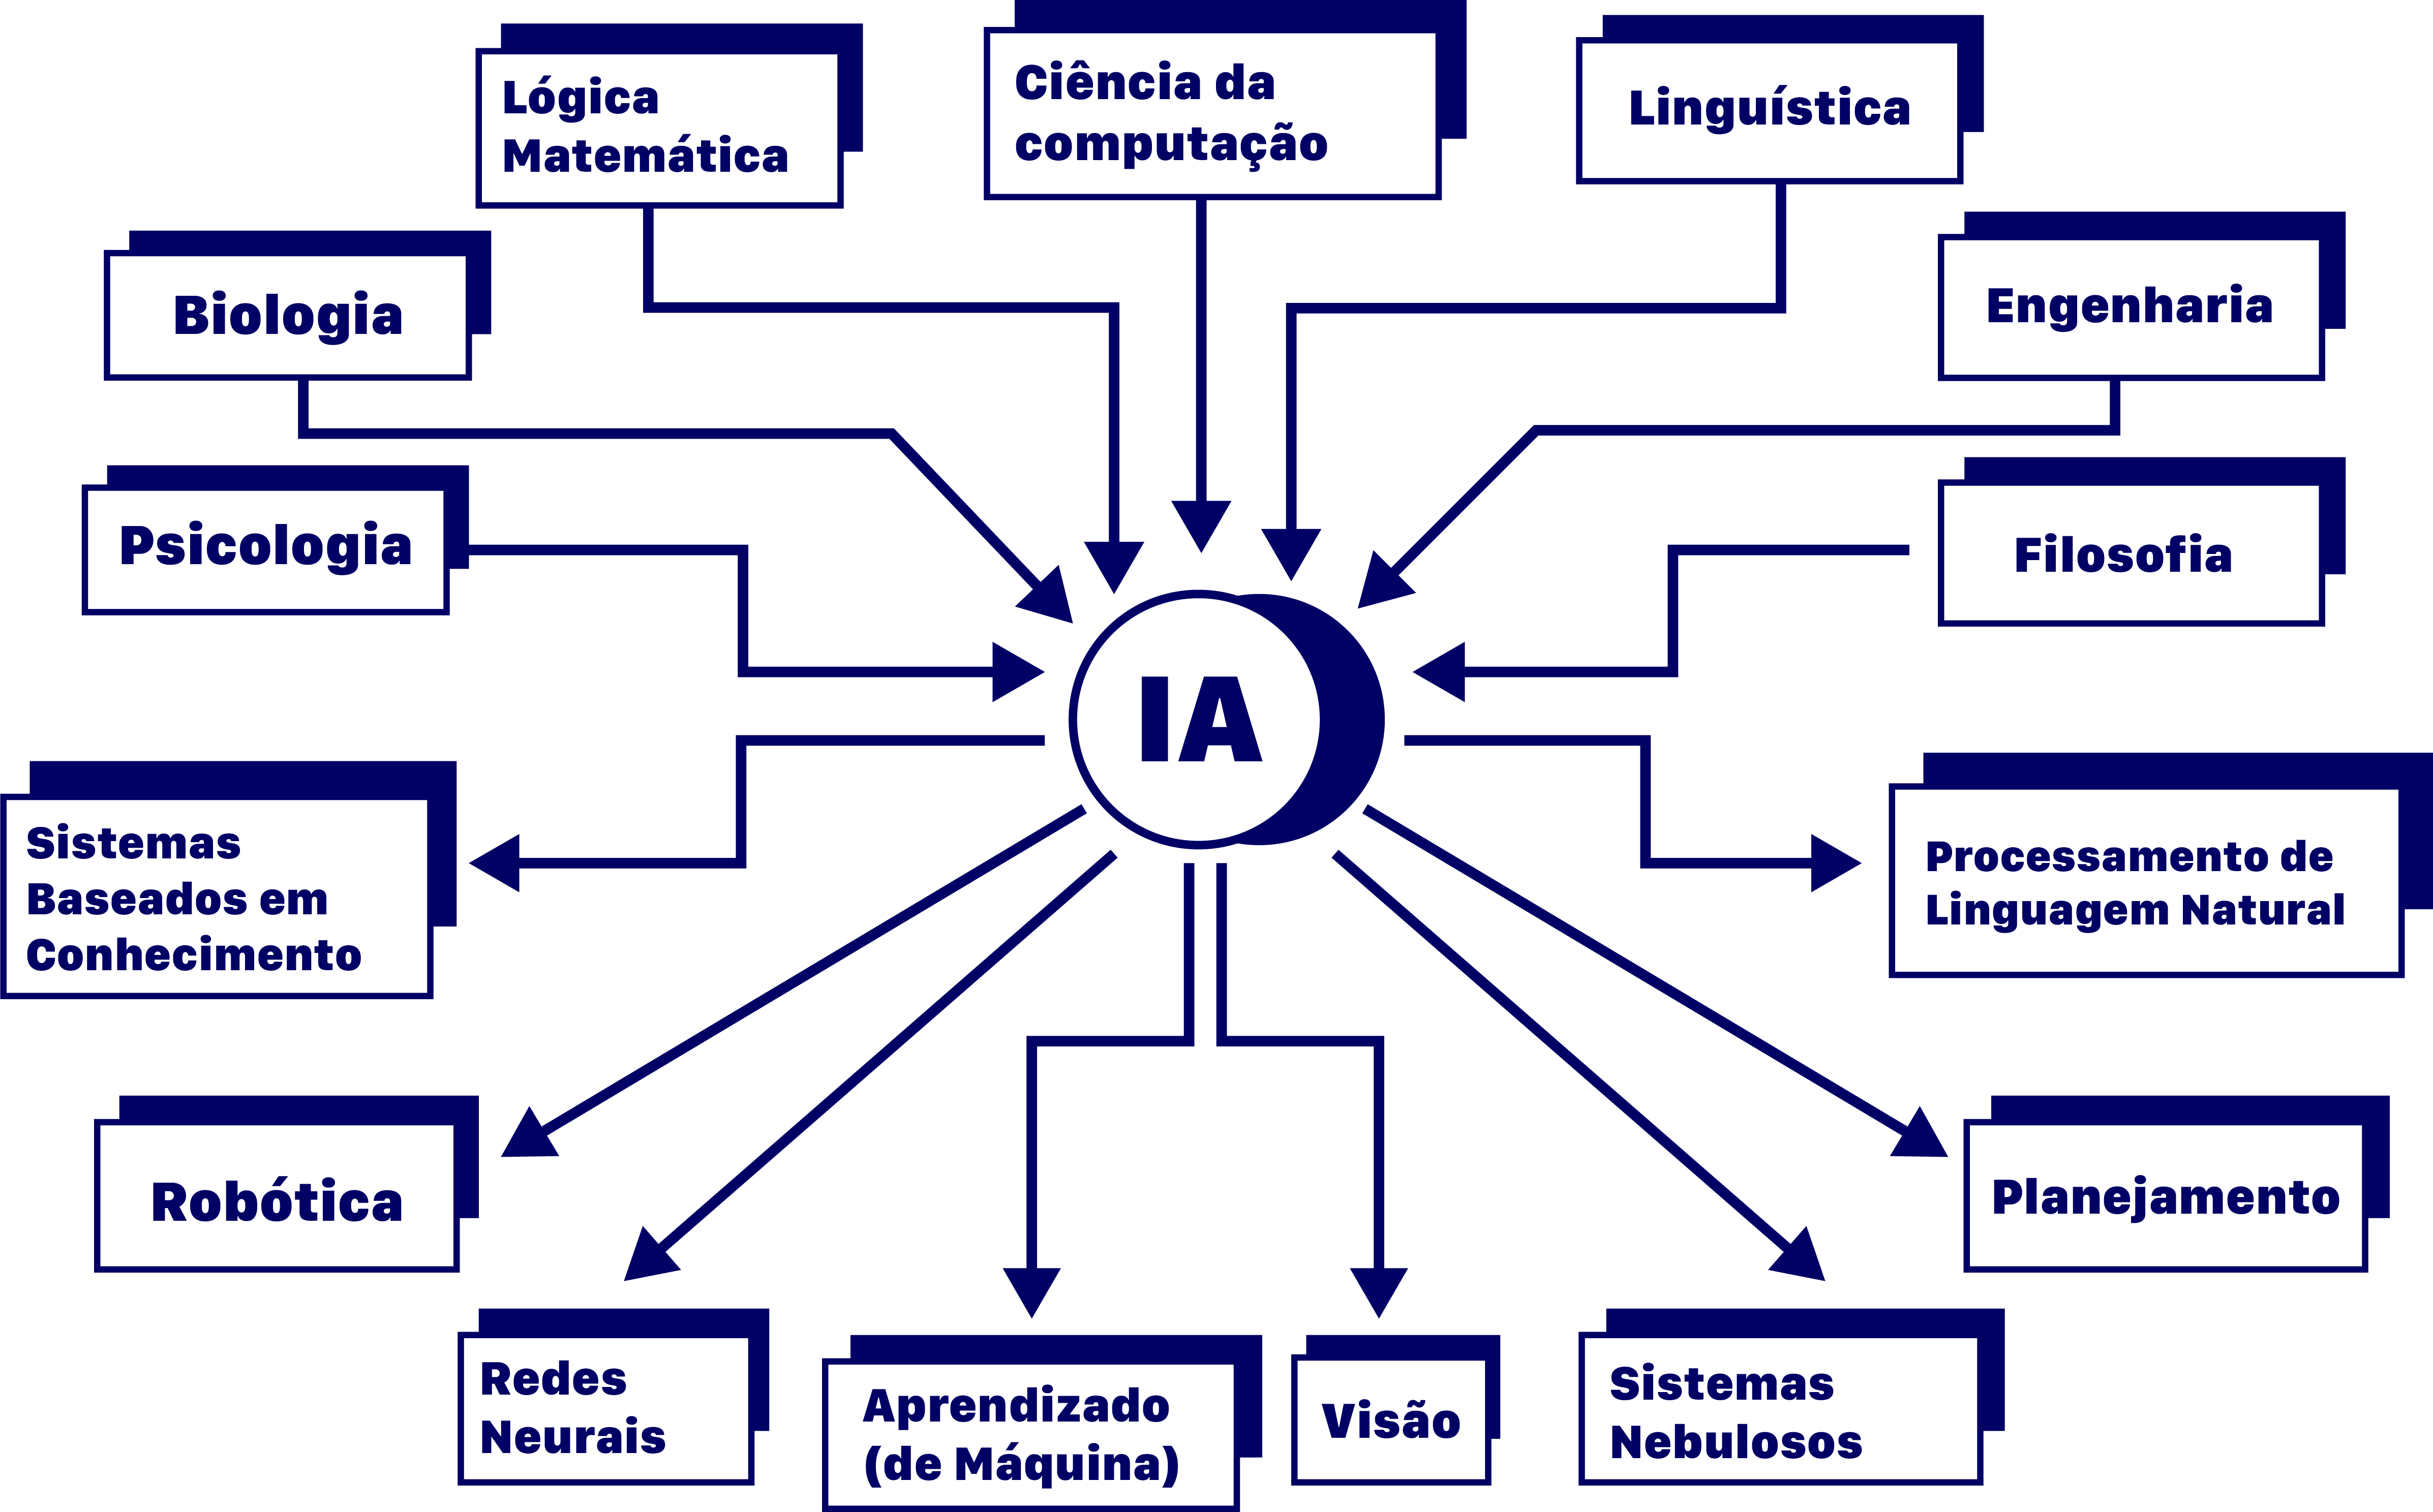
\includegraphics[width=10cm]{figures/areas_ia.png} % leia abaixo
% 	\legend{Fonte: \citeonline{aplicacoes_ia_vg}}
% 	\label{fig:areas_ia}
% \end{figure}

A ideia geral de inteligência artificial foi apresentado primordialmente no artigo de Alan Turing — conhecido como pai da computação — denominado de \textit{Computing Machinery and Intelligence} em 1950, outro conceito apresentado também foi o Teste de Turing, uma série de questionamentos que visa provar se a máquina pode executar um comportamento inteligente semelhante ao ser humano \space\cite{NationalGeographic2023}.

As aplicações de IA são várias, sendo algumas: controlar estoques de produtos nas empresas tanto na logística interna como externa, dirigir carros de forma autônoma, reconhecimento facial com base em vídeos ou fotos, criar imagens com base em um texto como na \cref{fig:ia_concept} — essa image foi gerada a partir da entrada: Um robô futurista com design elegante e moderno, sentado em uma cadeira enquanto lê um livro sobre inteligência artificial. O robô tem um olhar pensativo e curioso enquanto aprende sobre o assunto —, uma imagem criada usando plataforma DALL·E e até mesmo classificar em imagens, objetos e/ou píxeis na área de segmentação \space\cite{Stefanini, OpenAI2021}.

\begin{figure}[ht]
	\caption{Imagem conceito de uma inteligencia artificial que é um robô humanoide}
	\centering % para centralizarmos a figura
	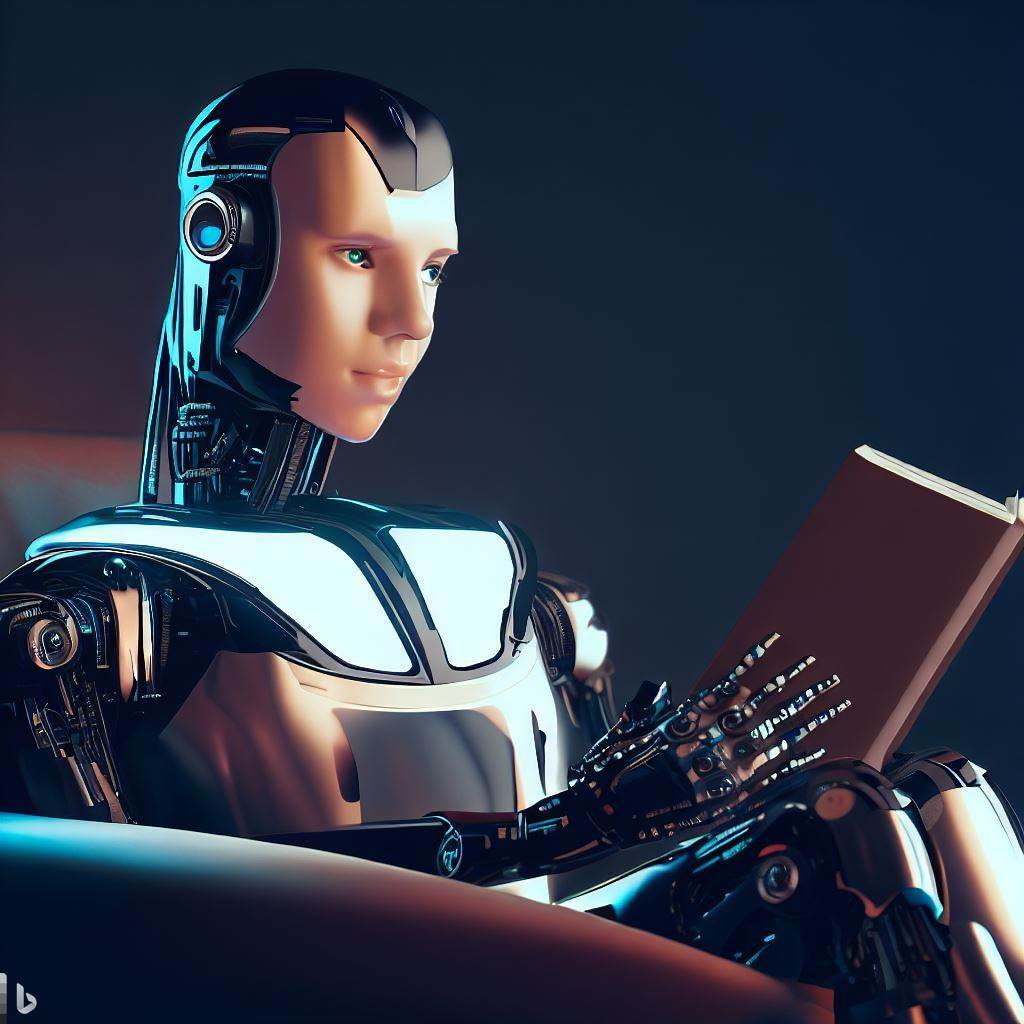
\includegraphics[width=6cm]{figures/ia_concept.jpg} % leia abaixo
	\legend{Fonte: DALL·E \citeonline{OpenAI2021}}
	\label{fig:ia_concept}
\end{figure}

% Segundo \citeonline{dp_overview} existem três principais tópicos sobre inteligência artificial, sendo eles: inteligência artificial, aprendizado de máquina e aprendizado profundo como mostrado na \cref{fig:diagrama_ia_ml_dp}.

% \begin{figure}[ht]
% 	\caption{Diagrama de Venn sobre relação entre os tópicos de inteligência artificial}
% 	\centering % para centralizarmos a figura
% 	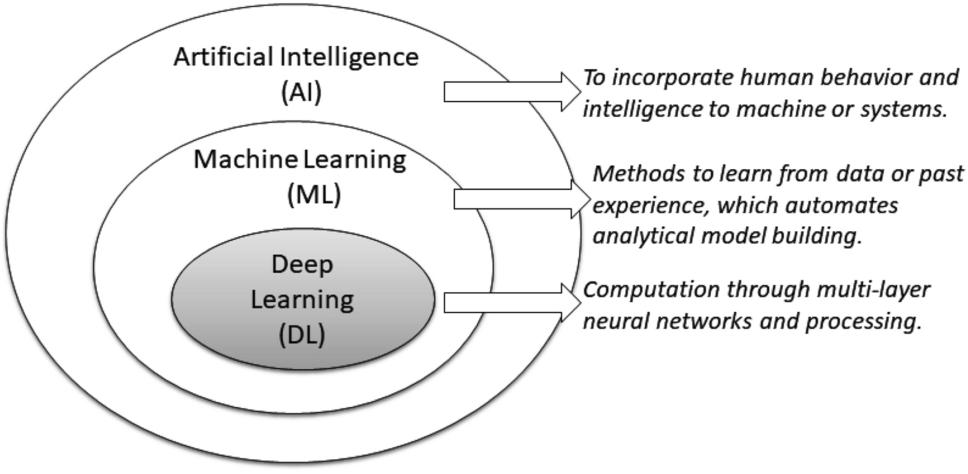
\includegraphics[width=10cm]{figures/diagrama_ia_ml_dp.png} % leia abaixo
% 	\legend{Fonte: \citeonline{dp_overview}}
% 	\label{fig:diagrama_ia_ml_dp}
% \end{figure}

